\documentclass[14pt]{extreport}
\usepackage{fontspec}
\usepackage{polyglossia}
\usepackage{graphicx}
\usepackage{hyperref}
\setmainlanguage{russian}
\setotherlanguages{english}
\setmainfont{Times New Roman}
\newfontfamily\cyrillicfont{Times New Roman}

\usepackage[a4paper,left=30mm,right=10mm,top=20mm,bottom=20mm]{geometry}
\setlength{\parindent}{1.25cm}
\setlength{\parskip}{0pt}
\linespread{1.5}

\begin{document}

    \title{Реферат на тему: \\[0.5cm] \textbf{Топ 5 лучших устройств вывода}}
    \author{Студент: Щеткин Дмитрий Сергеевич \\ Группа: 2.1}
    \date{17.09.2024}

    \maketitle
    
    \tableofcontents
    
    \chapter{Введение}
    В мире современных технологий устройства вывода играют ключевую роль, связывая нас с информацией и расширяя возможности взаимодействия с ней. 
    
    В этом списке представлены пять лучших устройств вывода, которые помогают нам взаимодействовать с технологиями каждый день. 
    
    \chapter{Топ устройств вывода}

    \section{ТОП - 5 Колонки}
    \begin{figure}[h]
        \centering
        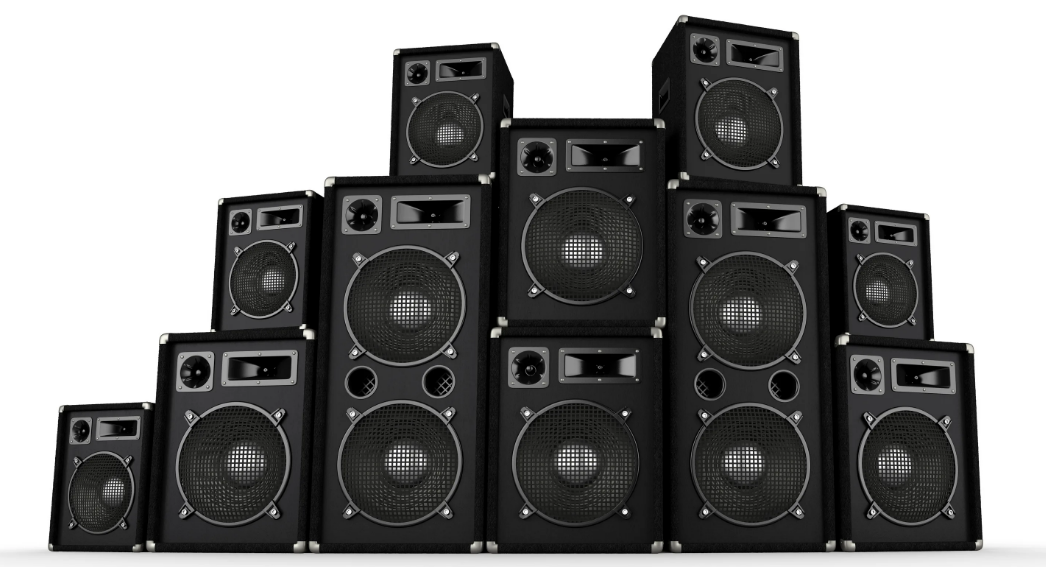
\includegraphics[width=0.5\textwidth]{kolonki.png}
        \caption{Колонки}
        \label{fig:example1}
    \end{figure}
        \begin{table}[h]
        \centering
        \begin{tabular}{|c|c|c|c|}
            \hline
            Модель & Тип & Мощность & Особенности \\
            \hline
            JBL Charge 4 & Портативная & 30 Вт & Водостойкость \\
            \hline
            Logitech Z906 & Стационарная & 500 Вт & Поддержка 5.1 звучания \\
            \hline
            Sony SRS-XB13 & Портативная & 10 Вт & Компактный размер \\
            \hline
            Marshall Stanmore & Стационарная & 80 Вт & Классический дизайн \\
            \hline
            Harman Kardon Aura & Стационарная & 60 Вт & 360° звучание \\
            \hline
        \end{tabular}
        \caption{Примеры колонок}
        \label{tab:example}
    \end{table}
    Колонки — это устройства вывода звука, которые позволяют воспроизводить музыку, аудио записи, а также озвучку видео. Современные колонки могут быть как стационарными, так и портативными, с поддержкой беспроводного подключения, что позволяет легко подключаться к телефону, ноутбуку или планшету.

    \section{ТОП - 4 \textit{Школьный} проектор}
    \begin{figure}[h]
        \centering
        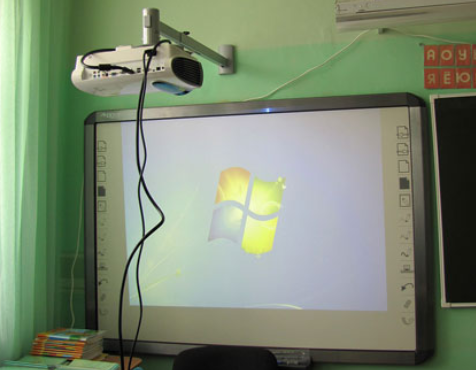
\includegraphics[width=0.5\textwidth]{proektor.png}
        \caption{Школьный проектор}
        \label{fig:example1}
    \end{figure}
    Школьный проектор — это удобное устройство для отображения учебного материала на большом экране. Современные проекторы могут подключаться к компьютерам и другим устройствам, обеспечивая высокое качество изображения и удобство использования.
    
    \section{ТОП - 3 Принтер}
    Принтер — это устройство вывода, которое позволяет создавать физические копии цифровых документов, изображений и других файлов.  Он незаменим в учебе и работе, так как помогает печатать текстовые материалы, рисунки, таблицы и презентации для удобного использования вне экрана.

    \subsection{Старый принтер}
    \begin{figure}[h]
        \centering
        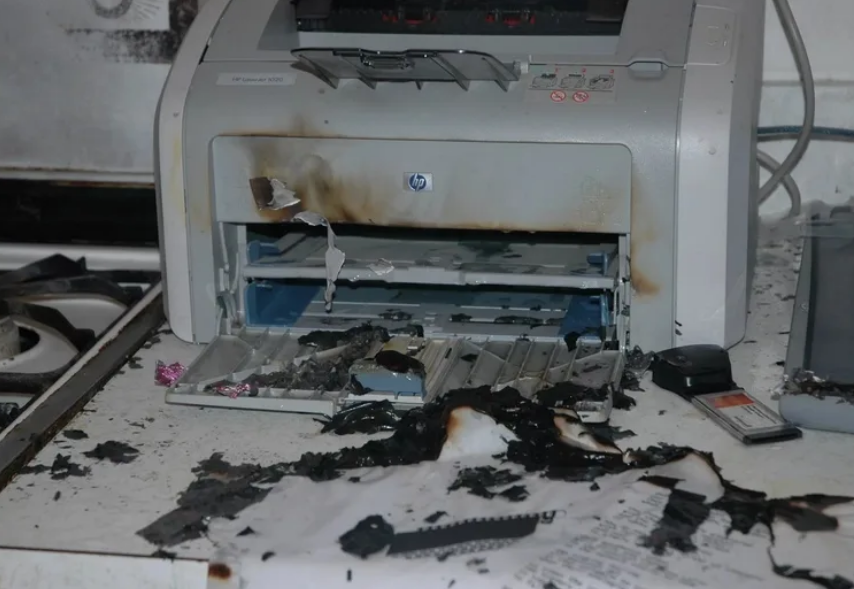
\includegraphics[width=0.5\textwidth]{printer.png}
        \caption{Старый принтер}
        \label{fig:example1}
    \end{figure}
    Старый принтер, хоть и медленный и шумный, когда-то был основным средством печати документов. Он требовал частой замены картриджей и подключения к компьютеру через кабель, но даже несмотря на эти неудобства, он служил верой и правдой, справляясь с основными задачами.

    \subsection{Новый принтер}
    \begin{figure}[h]
        \centering
        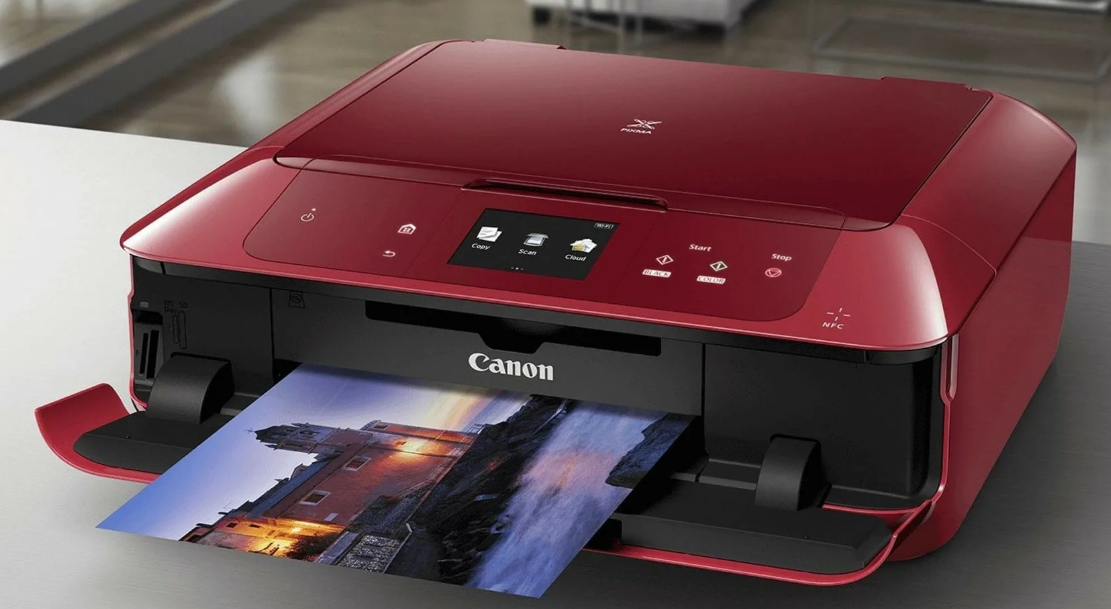
\includegraphics[width=0.5\textwidth]{printernovi.png}
        \caption{Новый принтер}
        \label{fig:example1}
    \end{figure}
    Новый принтер отличается высокой скоростью, бесшумной работой и возможностью беспроводного подключения. Благодаря современным функциям, этот принтер стал более экономичным и удобным в использовании, чем его предшественники.

    \section{ТОП - 2 Монитор}
    \begin{figure}[h]
        \centering
        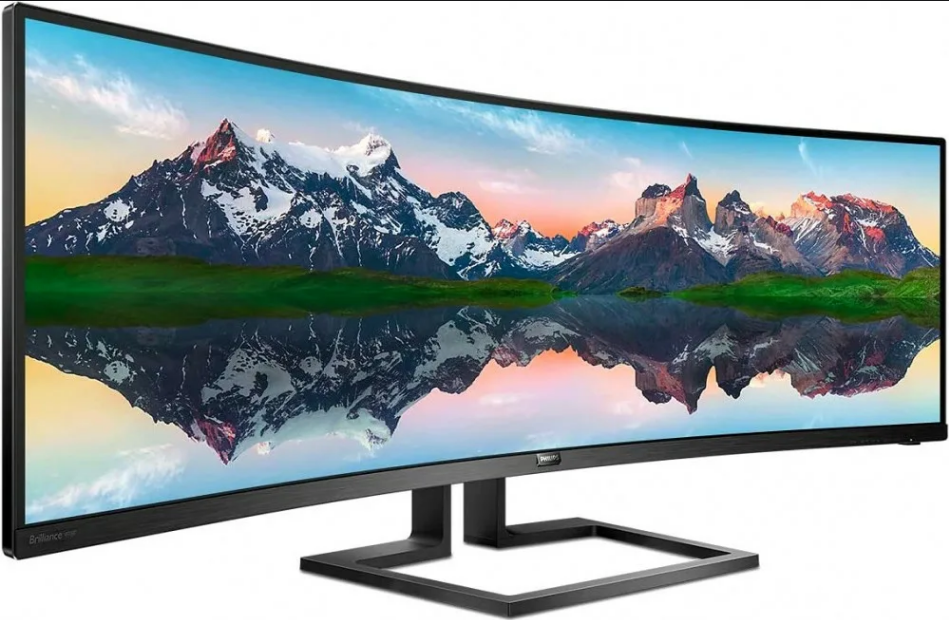
\includegraphics[width=0.5\textwidth]{monitor.png}
        \caption{Монитор}
        \label{fig:example1}
    \end{figure}
    Монитор — это основной визуальный интерфейс для взаимодействия с компьютером, который выводит информацию в виде текста, изображений и видео. В образовательной и рабочей среде мониторы обеспечивают комфортную работу с текстами, графикой и мультимедийными файлами. Современные мониторы обладают высоким разрешением и поддерживают широкий цветовой охват, что особенно полезно для дизайнеров и разработчиков.
    
    \begin{itemize}
        \item \textbf{ЭЛТ (CRT) мониторы} — использовали электронно-лучевые трубки для вывода изображения. Сегодня практически не применяются, так как заменены более современными технологиями.
        \item \textbf{ЖК (LCD) мониторы} — плоские дисплеи на основе жидкокристаллической технологии, отличаются малым весом, энергосбережением и хорошим качеством изображения.
        \item \textbf{Светодиодные (LED) мониторы} — это улучшенная версия ЖК-мониторов, где подсветка обеспечивается светодиодами, что повышает яркость и цветопередачу.
        \item \textbf{OLED мониторы} — используют органические светодиоды, обеспечивают высокую контрастность, насыщенность цветов и быстрый отклик, но могут быть дороже.
        \item \textbf{Изогнутые мониторы} — имеют изогнутую форму экрана, что помогает создавать эффект погружения и снижает искажения на краях.
        \item \textbf{Сенсорные мониторы} — поддерживают ввод с помощью касания, используются в информационных киосках, кассовых аппаратах и некоторых домашних компьютерах.
    \end{itemize}

    \section{ТОП - 1 Наушники}
    \begin{figure}[h]
        \centering
        
\includegraphics[width=0.5\textwidth]{nayshniki.png}
        \caption{Наушники}
        \label{fig:example1}
    \end{figure}
    Наушники — это одно из самых удобных и популярных устройств вывода звука, обеспечивающее личное погружение в аудиоматериалы. Они позволяют слушать музыку, смотреть видео или участвовать в звонках, не мешая окружающим. Современные наушники оснащены функциями шумоподавления, что улучшает качество звука, особенно в шумной среде.
    
    \chapter{Заключение}
    Таким образом, устройства вывода играют важнейшую роль в нашем взаимодействии с информацией, делая её более доступной, наглядной и удобной для восприятия. От качественного звука в наушниках до ярких изображений на экране монитора — каждое из них имеет свои особенности и преимущества, подходящие для различных задач. Благодаря таким устройствам, как проекторы, принтеры и колонки, мы можем более эффективно учиться, работать и наслаждаться развлечениями. Выбирая подходящие устройства вывода, мы не только улучшаем качество взаимодействия с технологиями, но и создаем комфортное пространство для учебы, работы и отдыха.
    
    \chapter{Список литературы}
    \begin{enumerate}
    \item \href{https://academia-moscow.ru/ftp_share/_books/fragments/fragment_19864.pdf}{Н.Н. Горнец, А.Г. Рощин, "ЭВМ и ПЕРИФЕРИЙНЫе УСТРОЙСТВА \\ Устройства ввода-вывода", Издательский центр «Академия» 2013.}
    \item  \href{https://scienceforum.ru/2019/article/2018010779}{А.М Сеферов, "Устройства вывода, их классификация и характеристики", ФБГОУ ВО ТюмИУ, 2019.}
    \end{enumerate}

\end{document}
